\section{课题主要研究内容及进度}
\subsection{课题主要研究内容}
近年来, 图像识别领域中深度神经网络被广泛使用。与之伴随的隐私问题也逐渐受到人们的关注。本课题主要关注图像识别领域中的两类比较有代表性的模型, 探讨其相关的隐私泄露问题。

第一类模型是基于模板(Template)匹配的识别模型, 主要应用于人脸识别、指纹识别等生物特征识别系统。此类模型用户的原始数据如人脸图像 $x$ , 经过特征提取网络 $F(\cdot)$ 得到特征模板 $t = F(x)$, 并存储于数据库, 这里的 $t$ 称为模板信息。在需要进行身份验证时, 用户给出新的输入图像 $x'$ ; 识别系统会比对此次输入的图像与数据库中的特征模板的匹配程度, 从而判断用户身份。以常见的余弦相似度为例, 模板匹配的判定准则为:
\[
  d(F(x'), t) = \frac{F(x') \cdot t}{\| F(x') \|_2 \| t \|_2}
\]
若 $d(F(x'), t) > \tau$, 则判定 $x'$ 与模板 $t$ 属于同一身份, 其中 $\tau$ 为系统设定的阈值。

虽然这种方法在实际应用中具有较高的准确率和效率, 但也存在隐私泄露的风险。具体来说, 由于模板存储在特征数据库中, 假设攻击者获得了特征数据库的访问权限, 窃取到特征模板信息, 则攻击者可以通过模板信息反向生成出接近用户的图像信息, 从而误导识别模型的识别结果。针对这类模型的攻击方法称为模板逆向攻击(Template Inversion Attack, TIA)。模板逆向攻击的核心在于利用特征模板 $t$ 来重建与之匹配的原始输入图像 $x'$ 。攻击者可以通过优化算法或生成模型来实现这一目标。此类攻击寻找一个输入 $x^*$, 使得其特征 $F(x^*)$ 与模板 $t$ 的相似度最大化, 可通过如下优化目标来描述:
$$x^* = \arg\min_{x'}Sim(F(x'), t)$$
其中$Sim(\cdot)$表示衡量特征与模板之间相似程度的函数。

%%%%%%%%%%%%%%%%%%%%%%%%%%%%%%%%%%%%%%%%%%%%%%%%%%%%%%%%%%%%%%%%%%%%%%%%%%%%%%%%%%%%%%%

第二类模型是图像分类模型, 主要应用于图像分类、目标检测等任务。此类模型通常包含与基于模板匹配的模型类似的提取特征的网络层, 与其不同之处在于图像分类模型在提取特征后包含额外的全连接层, 将提取的特征值转化为置信度分布, 输出每个类别的概率分布, 以此来达到分类的目的。图像分类模型的工作流程可以分为三个步骤: (1)输入图像 $x$ 经过特征提取网络 $f(\cdot)$, 得到特征向量 $t = f(x)$; (2)特征向量 $t$ 经过全连接层和激活函数, 输出类别概率分布 $p = g(t)$; (3)根据最大概率进行分类决策 $\hat{y} = \arg\max p$。

针对此类模型, 攻击者的目的是通过对模型参数的分析, 推断出训练数据的分布和特征, 从而恢复用户的隐私信息。与这类模型相关的攻击一般被称为模型反演攻击(Model Inversion Attack, MIA), 其目的是利用"目标分类器"来重构私有训练样本。在本课题中, 我们重点研究白盒情境下的模型反演攻击。在这种情况下, 攻击者被假设可以完全访问目标分类器, 攻击者拟定一个类别, 利用模型参数和训练数据的分布信息, 推断出训练该模型对应该类别训练所使用的图像。具体来说, 假设已知模型 $F$ 及其参数, 攻击者通过优化或生成方法, 寻找一个输入 $x^*$, 使得模型输出满足属于某一特定类别, 从而重建或推断出训练数据的敏感信息。设 $F(x)$ 为模型对输入 $x$ 的分类概率输出, $y_{t}$ 为目标类别。攻击者的目标是找到一个输入 $x^*$,使得模型 $F$ 在目标类别 $y_t$ 上的输出概率最大,即:
$$x^* = \arg\max_{x} \; P(y_t \mid x; F)$$

%%%%%%%%%%%%%%%%%%%%%%%%%%%%%%%%%%%%%%%%%%%%%%%%%%%%%%%%%%%%%%%%%%%%%%%%%%%%%%%%%%%%%%%

在目前已有的关于模板逆向攻击和模型反演攻击的研究中,较为流行的手段是利用生成模型来完成攻击任务。主要使用的生成模型可以分为两种: 一种是基于生成对抗网络(Generative Adversarial Networks, GAN)的生成模型, 另一种是基于扩散模型(Diffusion Models, DM)的生成模型。GAN通过对抗训练迫使生成器学习如何生成接近真实分布的图像, 而扩散模型则通过采样随机噪声并逐步去噪来重建图像。本课题将重点研究基于扩散模型的模板逆向攻击方法和模型反演攻击方法, 利用扩散模型强大的生成能力, 设计高效的模板逆向攻击和模型反演攻击算法。

本课题的研究中涉及的扩散模型主要基于明晰扩散模型(Elucidated Diffusion Models, EDM)的原理设计。EDM是扩散概率模型领域的重要进展, 由Karras等人在2022年提出。EDM对扩散过程的噪声调度、采样策略和损失函数进行了系统性分析和优化, 极大提升了扩散模型的采样效率和生成质量。

具体来说, 扩散模型通过逐步向数据添加噪声, 将数据分布映射为高斯分布, 并训练神经网络学习逆过程以去噪重建数据。EDM提出了一种统一的噪声调度框架, 定义了噪声幅度 $\sigma$ 的连续变化, 并用参数化的去噪器 $f_\theta(x, \sigma)$ 预测无噪声数据。EDM的核心训练目标为:
\[
  \mathcal{L}(\theta) = \mathbb{E}_{x_0, \sigma, \epsilon} \left[ w(\sigma) \left\| f_\theta(x_0 + \sigma \epsilon, \sigma) - x_0 \right\|^2 \right]
\]
其中, $x_0$ 为真实样本, $\epsilon \sim \mathcal{N}(0, I)$ 为高斯噪声, $\sigma$ 为噪声幅度, $w(\sigma)$ 为权重函数。


EDM的采样过程可用如下随机微分方程描述:
\[
  dx = -\frac{1}{2} \sigma^2 \nabla_x \log p_\theta(x, \sigma) \, d\sigma + \sigma \, dW
\]

其中 $dW$ 为维纳过程, $\nabla_x \log p_\theta(x, \sigma)$ 由神经网络近似。基于以上随机微分方, EDM提出使用二阶采样器来大幅减少采样步数, 提升生成速度。EDM框架统一了多种扩散模型的训练与采样方式, 便于理论分析和工程实现。本课题使用EDM扩散模型作为基础, 设计任务对应的生成模型来达到攻击目的。通过对EDM的训练和优化, 利用不同任务信息来重建匹配的原始输入图像, 从而实现对用户隐私信息的还原。

\subsection{进度介绍}
截至目前, 已完成课题相关的文献调研和相关理论的学习, 确定了研究方案, 搭建了实验环境。针对模板逆向攻击, 已实现了基于扩散模型的初步攻击方法, 并对其有效性进行了初步实验验证, 收集并分析了实验结果。

\section{目前已完成的主要研究工作及结果}

针对TIA和MIA的研究, 已完成以下工作:

(1)文献调研: 查阅了大量关于模板逆向攻击和模型反演攻击的相关文献, 了解了当前研究现状和技术难点。深入学习了图像识别模型的工作原理, 扩散模型数学原理以及加噪训练过程去噪生成过程。

(2)实验环境搭建: 搭建了实验所需的软硬件环境, 包括深度学习框架和必要的计算资源。

(3)研究方案设计: 设计了基于EDM扩散模型的模板逆向攻击和基于微调预训练换脸模型的模型反演攻击的研究方案, 明确了研究目标和方法。

(4)初步实现: 实现了基于EDM扩散模型的模板逆向攻击算法, 并对其进行了初步测试, 验证了其可行性, 并评估了攻击方法的有效性和生成图像的质量。

\subsection{模板逆向攻击的研究进展}
针对基于模板匹配模型的隐私泄露问题, 设计了如图\ref{fig:edm_tia_train}所示的利用EDM扩散模型进行模板逆向攻击的训练流程。其中扩散模型的核心部分采用了EDM扩散模型, 利用其生成能力和噪声调度机制, 实现高效的模板逆向攻击算法。通过对扩散模型的训练和优化, 模型可以重建与目标模板匹配的原始输入图像, 从而实现对用户隐私信息的还原。本课题在损失函数设计上, 结合了特征提取网络与扩散生成模型, 使得攻击流程能够同时优化生成图像的像素质量以及其与目标模板的特征相似度。

\begin{figure}[!htbp]
  \centering
  \includegraphics[width=0.7\textwidth]{images/train.drawio.pdf}
  \caption{基于EDM的模板逆向攻击模型训练流程示意图}
  \label{fig:edm_tia_train}
\end{figure}

%%%%%%%%%%%%%%%%%%%%%%%%%%%%%%%%

以EDM扩散模型为基础, 训练中使用的损失函数可以概括为:

\[
  \mathcal{L}(\theta) = \mathbb{E}_{x_0, \sigma, \epsilon} \left[ w(\sigma) \left\|  f_\theta(x_0 + \sigma \epsilon,y,\sigma) - x_0 \right\|^2 \right]
  + \lambda \| F( f_\theta(x_0 + \sigma \epsilon,y,\sigma)) - F(x_0) \|^2
\]

其中, $F(\cdot)$ 表示特征提取网络, $y$ 为目标类别标签, $\lambda$ 为平衡系数。损失函数由两部分组成: 第一项是像素空间的均方误差损失, 用于衡量生成图像与原始输入图像在像素级别上的相似度, 确保生成图像具备较高的视觉质量和基础结构还原能力; 第二项是特征空间的损失, 通过特征提取网络 $F$ 计算生成图像与原始图像在特征空间的距离, 用于衡量生成图像与目标模板之间的匹配程度, 从而提升攻击的有效性。$\lambda$ 的作用是平衡这两部分损失的影响, 使得模型在训练过程中既能生成与原始输入图像高度相似的图像, 又能保证生成图像在特征空间上与目标模板保持一致。

模板逆向攻击模型训练的具体步骤如算法\ref{alg:edm_tia_train}所示:

\begin{algorithm}[H]
  \caption{模板逆向攻击模型训练}
  \label{alg:edm_tia_train}
  \begin{algorithmic}[1]
    \REQUIRE 训练样本集 $\mathcal{D}$, 扩散生成模型 $f_\theta$, 特征提取网络 $F$
    \ENSURE 训练好的生成模型参数 $f_\theta$
    \FOR{迭代 $=1$ 到 $N$}
    \STATE 随机采样一批训练样本 $(x_0, y_0)$
    \FOR{每个样本 $(x_0, y_0)$}
    \STATE 采样噪声 $\epsilon \sim \mathcal{N}(0, I)$, 噪声幅度 $\sigma$
    \STATE 计算带噪输入 $x = x_0 + \sigma \epsilon$
    \STATE 生成图像 $\hat{x} = f_\theta(x, y_0, \sigma)$
    \STATE 计算损失
    \[
      \mathcal{L}(\theta) = \mathbb{E}_{x_0, \sigma, \epsilon} \left[ w(\sigma) \left\|  f_\theta(x_0 + \sigma \epsilon,y_0,\sigma) - x_0 \right\|^2 \right]
      + \lambda \| F( f_\theta(x_0 + \sigma \epsilon,y_0,\sigma)) - F(x_0) \|^2
    \]
    \ENDFOR
    \STATE 更新 $\theta$ 以最小化 $\mathcal{L}(\theta)$
    \ENDFOR
  \end{algorithmic}
\end{algorithm}


在训练完毕后, 模型可以用于推理阶段, 即利用训练好的扩散模型生成与目标特征模板匹配的图像。推理阶段的主要目标是, 在已知目标特征模板的情况下, 通过扩散模型逐步去噪, 从随机噪声中重建出与该模板高度匹配的原始输入图像。在实际采样时, 常用离散步长来近似EDM的随机微分方程采样过程, 即:
\[
  x_{i-1} = x_i + \frac{1}{2} \sigma_i^2 \nabla_x \log f_\theta(x_i, \sigma_i, y) \Delta \sigma + \sigma_i \sqrt{\Delta \sigma} \cdot z_i
\]

其中 $z_i \sim \mathcal{N}(0, I)$, $\Delta \sigma = \sigma_{i-1} - \sigma_i$。具体而言, 首先以随机噪声作为初始输入, 结合目标模板信息, 经过多步迭代的去噪过程, 模型不断优化生成图像的特征, 使其在特征空间中逐渐接近目标模板。每一步生成的中间结果都会被输入特征提取网络进行特征对齐, 确保最终生成的图像不仅在视觉上具有较高的质量, 同时在特征空间中与目标模板高度一致。图\ref{fig:edm_tia_infer}展示了扩散模型在模板逆向攻击中的应用过程。



\begin{figure}[!htbp]
  \centering
  \includegraphics[width=0.8\textwidth]{images/infer.drawio.pdf}
  \caption{基于EDM的模板逆向攻击模型推理流程示意图}
  \label{fig:edm_tia_infer}
\end{figure}

针对以上的训练流程和推理流程方案,本实验采用公开的人脸图像数据集 CelebA 作为基础数据集进行了初步试验。CelebA 数据集包含10177个不同身份的202599张人脸图像, 广泛应用于人脸识别和生成模型等相关研究。在攻击目标模型的选择上, 本课题采用了当前主流的人脸识别模型 ArcFace。ArcFace是一种基于残差网络结构的人脸识别模型, 通过引入角度间隔损失, 显著提升了特征的判别性和区分度。该模型能够将同一身份的特征向量聚集在一起, 同时有效拉开不同身份之间的特征距离, 从而在大规模人脸识别任务中实现更高的准确率。

数据集的准备工作包括对 CelebA 数据集进行预处理, 提取人脸图像特征并保存为数据对, 具体步骤如下:
(1)根据CelebA数据集的提供的人脸关键点信息, 对人脸图像进行裁剪和对齐, 调整图片尺寸为112, 确保人脸位于图像中心, 并且大小一致。
(2)使用ArcFace模型对每张图像进行特征提取, 得到对应的特征模板, 设置与图像的对应关系。
(3)将裁剪后的图像根据图像与人物类别的对应关系进行标注, 并根据人物类别不相交的原则, 将数据集划分为训练和测试数据集, 其中训练集包含9669个人物共192241张人脸图像, 测试集包含508个人物共10358张图像。

训练过程中, 为平衡生成图像与特征模板之间的相似度和生成图像与原始输入图像之间的相似度, 采用了动态的线性权重 $\lambda$。具体来说, 在训练的初期, $\lambda$ 的值较小, 以确保模型能够先学习到图像的基本结构和特征; 随着训练的进行, 逐渐增大 $\lambda$ 的值, 以增强生成图像与特征模板之间的匹配度。这样可以有效地提高生成图像的质量和与目标模板的相似度。实验中, $\lambda$ 的初始值设置为0, 并在训练过程中逐渐增加到100。具体的调整策略为: 模型每学习1000张图像, 将 $\lambda$ 增加0.01, 在10000次迭代后, 直到达到最大值100。

训练中损失函数变化如图\ref{fig:edm_template_attack_loss}所示:

\begin{figure}[htbp]
  \centering
  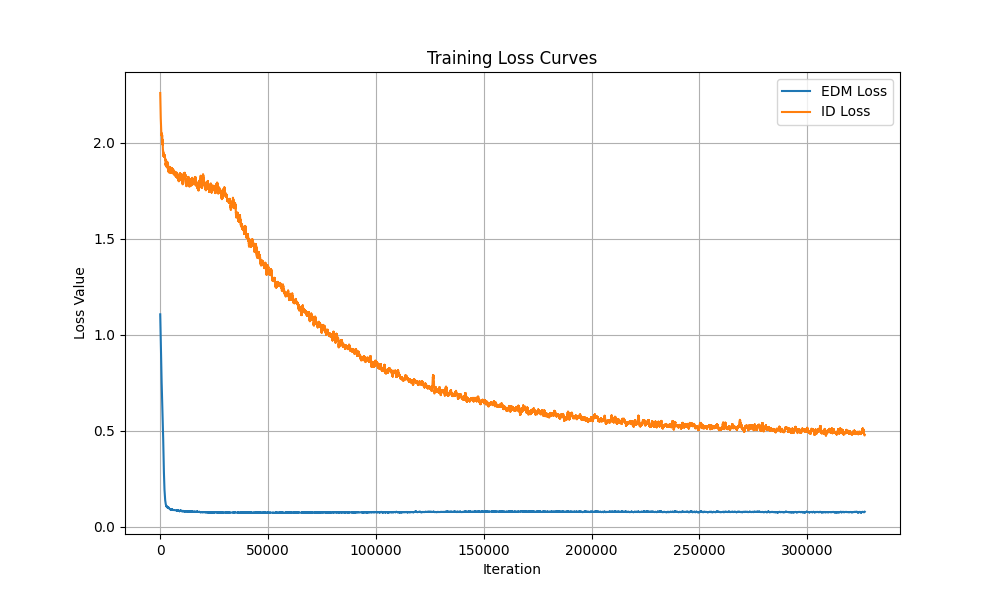
\includegraphics[width=0.8\textwidth]{images/loss_curve.png}
  \caption{基于EDM的模板逆向攻击训练过程损失函数变化曲线}
  \label{fig:edm_template_attack_loss}
\end{figure}

其中 $id\,loss$ 和 $EDM\,loss$ 分别表示模板信息一致性损失和图像重建的像素损失。由于$id\,loss$实际值较小, 图中将其放大了1000倍以便于观察。可以看出, 随着训练的进行, 图像重建的像素损失先于模板信息一致性损失收敛, 表明模型在学习过程中首先关注的是还原人脸图像的基础结构和像素细节, 使生成图像能够在视觉上与原始图像保持较高的一致性。随着训练的深入, $\lambda$逐渐增加, 模型的优化重心逐渐转向提升生成图像与目标特征模板之间的匹配度。此时, 模板信息一致性损失开始显著下降, 模型不断学习如何更好地捕捉和还原与目标身份相关的深层特征。整体来看, 损失函数的变化趋势反映了模型从低层像素信息到高层语义特征的逐步学习过程。

在模板逆向攻击的推理阶段, 使用训练好的EDM扩散模型对测试集中的特征模板进行攻击。首先, 从分割好的测试集中随机选取1000个特征模板, 构建隐私数据库。随后, 将这些特征模板作为条件输入, 引导EDM扩散模型进行图像生成。

采样过程中, 参数设置如下: 迭代次数$steps = 18$,
终止点噪声幅度$\sigma_{\text{min}} = 0.002$,初始点噪声幅度$\sigma_{\text{max}} = 80$, 噪声调度参数$\rho = 7 $, 采样范围参数$S_{\text{churn}} = 0$, $S_{\text{min}} = 0$, $S_{\text{max}} = \infty$, 噪声扰动参数$S_{\text{noise}} = 1$。这些参数的选择基于EDM扩散模型的设计原则, 旨在平衡生成图像的多样性和质量。

生成的图像随后输入ArcFace模型进行特征提取, 并与隐私数据库中的特征模板进行匹配。通过计算生成图像特征与目标模板的相似度, 若相似度高于设定阈值(根据系统精度需求设定, 实验中采用0.5), 则认为该生成图像成功重建了与目标模板匹配的原始输入图像。

% - **迭代次数(steps=18)**: 扩散模型在生成图像时进行的去噪步数, 步数越多, 生成图像质量通常越高, 但计算量也越大。
% - **sigma_min=0.002**: 扩散过程中的最小噪声幅度, 决定了去噪的终止点, 影响最终生成图像的细节还原。
% - **sigma_max=80**: 扩散过程中的最大噪声幅度, 决定了初始噪声的强度, 影响生成过程的多样性。
% - **rho=7**: 控制噪声调度的参数, 影响噪声幅度在采样过程中的变化速率。
% - **S_churn=0**、**S_min=0**、**S_max=float("inf")**、**S_noise=1**: 这些参数用于进一步调节采样过程中的噪声扰动和采样范围, 通常用于提升生成图像的多样性和稳定性。

实验结果显示, 所提出的方法在模板逆向攻击任务中取得了较高的攻击准确率, 达到92\%。这表明生成的图像能够有效地欺骗目标识别模型, 使其输出与目标模板高度一致的特征。部分生成图像如图\ref{fig:edm_tia_sample}所示。可以看出, 所提出的方法能够有效地重建与目标特征模板相匹配的人脸图像。生成的人脸图像在整体结构、面部特征等方面与原始输入图像高度相似, 且具备较高的视觉质量, 但部分生成图像存在图像模糊、细节缺失等现象, 需要进一步提升效果。生成图像的质量评价指标结果如表\ref{tab:quality_metrics}所示。

\begin{figure}[!htbp]
  \centering
  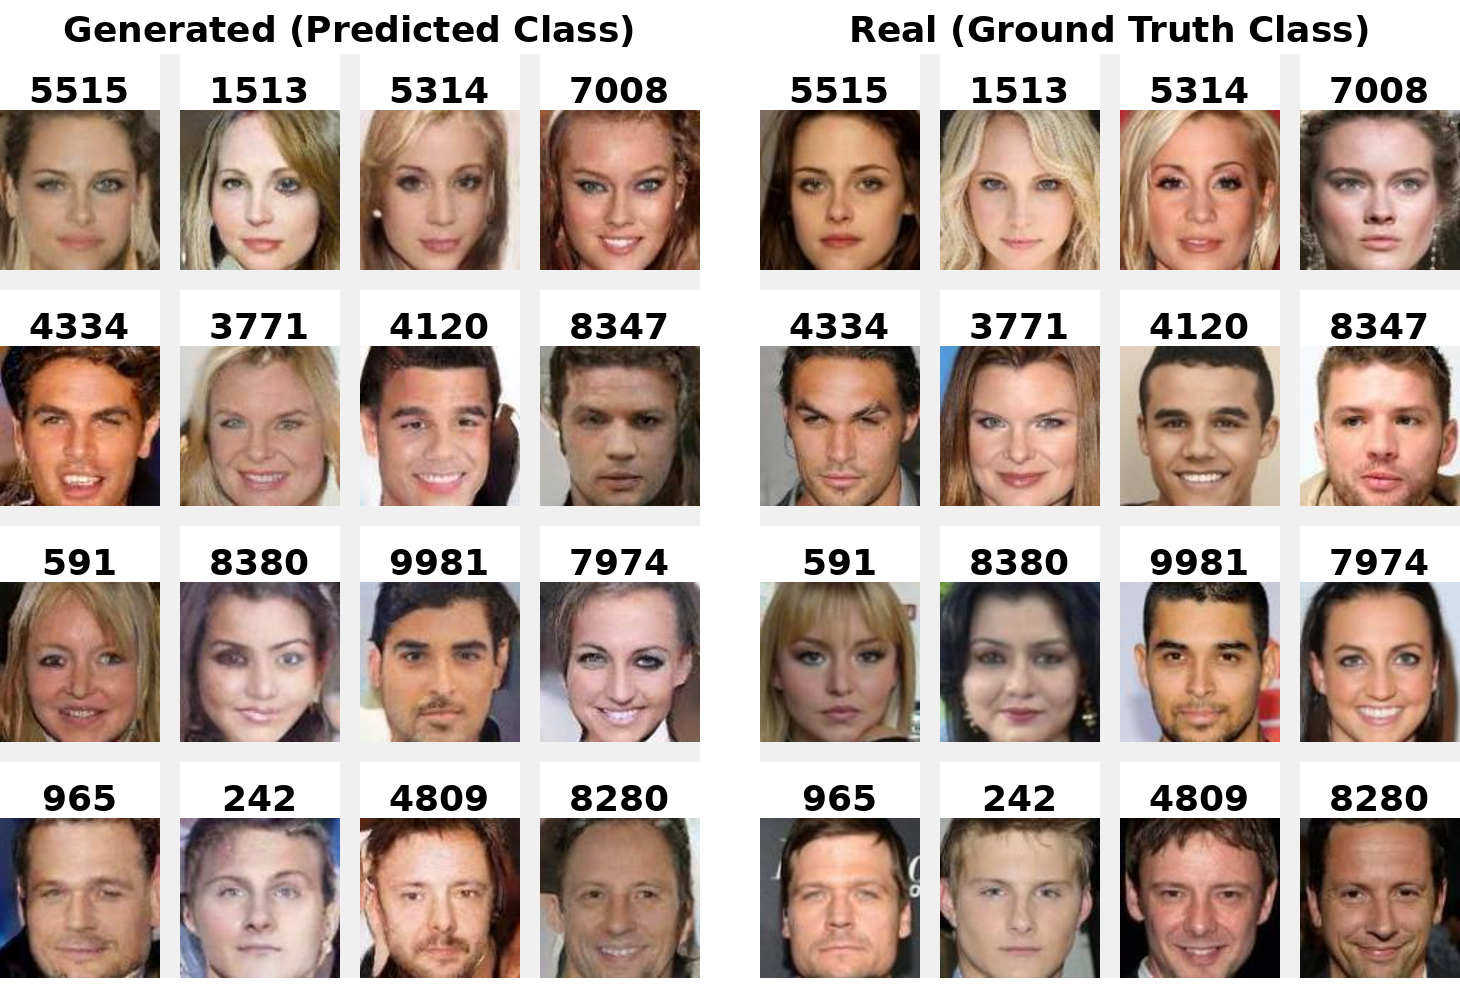
\includegraphics[width=0.8\textwidth]{images/gen_vs_real_matrix.png}
  \caption{模板逆向攻击生成图像与真实图像对比样例}
  \label{fig:edm_tia_sample}
\end{figure}

\begin{table}[htbp]
  \centering
  \begin{tabular}{lc}
    \hline
    指标         & 数值              \\
    \hline
    FID        & 22.3193         \\
    KID        & 0.0075 ± 0.0005 \\
    LPIPS Alex & 0.3129          \\
    LPIPS Vgg  & 0.4854          \\
    \hline
  \end{tabular}
  \caption{各项图像质量评价指标结果}
  \label{tab:quality_metrics}
\end{table}

% LPIPS (alex): 0.31297400742024184
% LPIPS (vgg): 0.48543246793746947
% Frechet Inception Distance: 22.31930493655588
% Kernel Inception Distance: 0.007591125510510506 ± 0.0005495588712487208


\subsection{模板逆向攻击的后续研究方案}
\label{sec:tia_finetune}

上述研究结果表明, 在训练模型中, 使用模板信息一致性损失和图像重建的像素损失一起训练, 随着动态权重的增加, 图像质量存在一定的下滑现象, 因此在已有的模板逆向攻击的基础上, 本课题进一步提出了一种基于一致性微调的两阶段训练策略。该策略旨在最大程度地保持生成图像的高质量, 同时引导模型生成与目标类别特征分布相匹配的图像。通过两阶段的训练策略, 预期模型不仅能够生成高质量、结构一致的图像, 还能进一步提升生成图像与目标类别特征的匹配度。整个训练过程如图\ref{fig:consistency_finetune}所示.

第一阶段为 EDM 核心损失训练, 主要目标是使生成模型能够充分学习数据的基础分布和图像生成的核心特征。在该阶段, 优化的损失函数为EDM的像素误差损失:

\[
  \mathcal{L}_{\text{EDM}}(\theta) = \mathbb{E}_{x_0, \sigma, \epsilon} \left[ w(\sigma) \left\| f_\theta(x_0 + \sigma \epsilon, t, \sigma) - x_0 \right\|^2 \right]
\]

其中, $x_0$ 表示原始图像, $\sigma$ 为噪声幅度, $\epsilon$ 为高斯噪声, $w(\sigma)$ 为噪声权重, $f_\theta$ 为生成模型。该阶段训练的重点在于提升生成图像的整体质量和结构一致性, 确保生成结果具备较高的真实性和清晰度。

第二阶段为微调阶段, 此时冻结大部分网络层, 仅对部分关键层进行微调。微调过程中, 引入模板信息一致性损失, 引导模型生成与目标模板信息特征更为匹配的图像。此阶段的损失函数可以使用特征值的均方误差损失来约束特征值的一致性:

\[
  \mathcal{L}_{id} = \| F( f_\theta(x_0 + \sigma \epsilon,y_0,\sigma)) - F(x_0) \|^2
\]
% 在一致性微调策略下, 模型的训练过程分为两个阶段。第一阶段是EDM核心损失训练, 主要目标是使生成模型能够充分学习数据的基础分布和图像生成的核心特征。在这一阶段, 模型专注于生成图像的整体质量和结构一致性, 确保生成结果具备较高的真实性和清晰度。第二阶段是微调阶段, 此时冻结大部分网络层, 仅对部分关键层进行微调, 以保持已获得的高质量图像生成能力, 并进一步调整生成策略, 使生成图像能够更好地与目标类别的特征分布相匹配。整个训练过程如图\ref{fig:consistency_finetune}所示, 清晰地展示了两阶段训练和参数调整的流程。

\begin{figure}[htbp]
  \centering
  \includegraphics[width=0.6\textwidth]{images/train_finetune.pdf}
  \caption{加入一致性微调后的两阶段模板逆向攻击示意图}
  \label{fig:consistency_finetune}
\end{figure}


\subsection{模型反演攻击的研究进展}

针对模型反演攻击, 为提升生成图像的质量和多样性, 在此方法的研究中引入基于换脸(Deepfake)技术的先验模型。这类模型利用深度学习方法对人脸图像的结构、纹理和表情等特征进行建模, 通过大量真实人脸数据的训练, 能够学习到人脸在不同身份、姿态和光照条件下的变化规律。换脸模型具备较强的图像生成与特征迁移能力, 可以将目标身份的特征融合到源图像中, 实现高质量的人脸合成。作为先验模型应用于生成任务时, 能够为后续的图像生成过程提供丰富的人脸先验知识, 提升生成图像的真实性和多样性, 并增强模型对目标特征的适应能力。

本课题将换脸模型应用到模型反演攻击中, 只需要在预训练的换脸模型的基础上, 对生成模型进行微调, 使其在保持原有生成能力的同时, 更好地适应目标分类模型的特征分布。微调过程中, 生成模型不仅学习到数据的通用特征, 还能够针对目标任务优化其生成过程, 从而提升生成图像与目标类别之间的匹配度。通过这种方式, 生成模型能够生成既符合真实分布、又与目标特征高度一致的图像, 可以有效提升了模板逆向攻击的成功率和生成样本的视觉质量。

本课题采用基于换脸模型作为先验模型的另一个优势在于其具备的灵活性和可控性。具体来说,假设攻击目标需要生成具有特定人脸姿态、表情或其他属性的图像,换脸模型能够通过调整输入的待替换人脸图像的姿态、表情、光照等因素,灵活地控制最终生成图像的外观特征。例如,在某些实际攻击场景中,攻击者可能希望生成一张带有特定微笑、侧脸或特定视角的人脸图像,以更好地适应目标系统的识别条件或满足特定的攻击需求。基于换脸技术的生成模型能够有效地融合目标身份的特征与输入人脸的姿态和表情,从而实现对生成图像的精细化控制。此外,这种灵活性不仅提升了生成模型在多样化攻击场景下的适应能力,还为攻击者提供了更多的操作空间,使其能够针对不同的目标和应用需求,定制化地生成符合要求的伪造图像。

本课题目前已经完成了训练流程和推理流程研究方案的设计。模型反演攻击的训练流程如图\ref{fig:edm_mia_train}所示:

\begin{figure}[!htbp]
  \centering
  \includegraphics[width=0.7\textwidth]{images/train_mia.drawio.pdf}
  \caption{基于换脸生成模型的模型反演攻击训练流程示意图}
  \label{fig:edm_mia_train}
\end{figure}

具体来说, 模型反演攻击中所采用的生成模型骨干结构为选定的预训练换脸模型, 并在其基础上增加标签嵌入层以实现通过分类标签控制的条件生成。在模型的训练阶段, 与\ref{sec:tia_finetune}节中的微调策略类似, 本课题将换脸模型的部分主干层参数冻结, 仅对标签嵌入层及部分生成层进行训练, 以兼顾生成能力与任务适应性。

训练流程可用算法\ref{alg:edm_mia_train}表示: 首先, 给定一张原始图像 $x$, 利用攻击目标的分类模型 $F$ 提取其分类标签 $y = F(x)$。随后, 将标签 $y$ 通过嵌入层映射为条件向量, 与原始图像一同输入到换脸生成模型 $f_{\theta}$, 生成伪造图像 $x' = f_{\theta}(x_0, y)$。生成的图像 $x'$ 再次输入分类模型 $F$, 获得预测标签 $y' = F(x')$。训练目标$\mathcal{L}_{Classification}$是最大化 $x'$ 被分类为目标标签 $y$ 的概率。

\begin{algorithm}[H]
  \caption{模型反演攻击训练流程}
  \label{alg:edm_mia_train}
  \begin{algorithmic}[1]
    \REQUIRE 训练样本集 $\mathcal{D}$, 预训练换脸生成模型 $f_\theta$, 目标分类模型 $F$
    \ENSURE 微调后的换脸生成模型 $f_\theta$
    \FOR{迭代 $=1$ 到 $N$}
    \STATE 随机采样训练样本 $x$ 作为待重建人脸, $x_0$ 作为待替换人脸图像
    \FOR{每个样本 $x$}
    \STATE 计算标签 $y = F(x)$
    \STATE 生成伪造图像 $x' = f_\theta(x_0, y)$
    \STATE 预测标签 $y' = F(x')$
    \STATE 计算分类损失 $\mathcal{L}_{\text{Classification}}(y', y)$
    \ENDFOR
    \STATE 更新 $f_\theta$ 以最小化 $\mathcal{L}_{\text{Classification}}$
    \ENDFOR
  \end{algorithmic}
\end{algorithm}

通过以上训练流程, 生成模型能够学习到如何根据目标标签生成与原始图像结构相似、且被目标分类器判别为指定类别的伪造图像, 从而实现对训练数据隐私的有效还原和攻击。

在模型反演攻击的推理流程中, 攻击者所掌握的信息仅限于目标类别标签, 相较于模板逆向攻击, 能够提供给生成模型的先验信息更为有限。因此, 推理过程中需要通过多次迭代, 不断生成图像并根据模型输出的置信度标签进行反馈优化, 直至生成的图像能够满足目标类别的要求。

整个推理流程如图\ref{fig:edm_mia_infer}所示。推理流程首先以一张初始人脸图像 $x_{\text{input}}$ 作为输入,攻击者可以根据任务需求灵活控制该输入人脸的姿态、表情等属性,以适应不同的攻击场景。在每一次迭代生成过程中,当前生成的图像 $x'$ 会被输入到目标分类模型 $F$ 中,获得其在各类别上的置信度分布 $y' = F(x')$。随后,根据分类模型输出的置信度结果,判断当前生成图像是否已经达到预设的目标类别 $y_t$ 的要求。具体而言,若 $y'_t = F(x') \geq \tau$,其中 $\tau$ 为设定的置信度阈值,则认为生成的图像已经满足目标要求,停止迭代。

如果当前生成的图像尚未达到目标类别的置信度要求,则进行下一轮迭代。根据本轮迭代图像分类损失 $\mathcal{L}_{\text{cls}}(y', y_t)$ 的梯度信息,引导$x'$修改, 形成新的$x_{input}$,作为下一轮迭代的人脸图像输入, 以进一步提升目标类别的置信度。该优化过程不断循环,持续迭代,直到生成的图像在目标类别上的置信度超过设定阈值,或达到最大迭代次数为止。通过这种反馈优化机制,能够有效地引导生成模型逐步生成与目标类别高度匹配的图像,从而提升模型反演攻击的成功率和生成样本的质量。

\begin{figure}[!htbp]
  \centering
  \includegraphics[width=0.8\textwidth]{images/infer_mia.drawio.pdf}
  \caption{模型反演攻击推理流程示意图}
  \label{fig:edm_mia_infer}
\end{figure}

\section{后期拟完成的研究工作及进度安排}
\subsection{后期拟完成的研究工作}

后期拟完成的研究工作主要包括以下几个方面:

(1) 设计结合换脸生成模型的模型反演攻击方法。本课题计划深入研究如何将预训练的换脸生成模型应用于模型反演攻击任务。具体而言,将充分利用换脸模型在高质量人脸生成方面的能力,通过对其进行针对性微调,使其更好地适应当前攻击任务的需求。研究重点包括:如何结合目标分类模型的输出信息,设计有效的优化算法,逐步重建与目标类别高度匹配的原始输入图像;以及如何构建合理的损失函数,充分利用目标模型的梯度信息和置信度标签,提升攻击的准确性和生成图像的真实性。

(2) 完善模板逆向攻击的训练方案,调整为二阶段训练方案,增加一致性微调步骤。  针对模板逆向攻击方法,后续将对现有的训练流程进行优化,采用两阶段训练策略。第一阶段侧重于生成模型的基础能力训练,确保生成图像具备较高的视觉质量和结构一致性;第二阶段则引入一致性微调步骤,冻结大部分网络层,仅对关键层进行微调,进一步提升生成图像与目标模板在特征空间中的匹配度。通过这种分阶段训练方式,有望显著提高模板匹配的准确性和生成图片的整体质量。

(3) 对模板逆向攻击和模型反演攻击进行大规模比对实验。为全面评估所提出方法的有效性和适用性,计划在多个公开数据集和不同目标模型下,开展大规模的对比实验。系统地比较模板逆向攻击与模型反演攻击在不同场景下的攻击效果。

(4) 撰写学位论文,整理研究成果,归纳总结隐私泄露问题。在完成上述研究工作的基础上,系统整理和归纳研究成果,撰写高质量的学术论文,全面总结本课题所提出的模板逆向攻击和模型反演攻击方法。


\subsection{后期进度安排}

根据后期拟完成的研究工作, 进度安排如表\ref{tab:progress_schedule}所示:
\begin{table}[H]
  \centering
  \begin{tabular}{lc}
    \hline
    时间节点     & 主要任务                           \\
    \hline
    2025年07月 & 设计模型反演攻击, 实现一致性微调方案和模型反演攻击方法   \\
    \hline
    2025年08月 & 进行实验并分析结果, 优化模型结果              \\
    \hline
    2025年09月 & 进行大规模实验, 验证两种攻击在不同数据集和模型架构下的效果 \\
    \hline
    2025年11月 & 撰写论文初稿                         \\
    \hline
    2025年12月 & 完善论文, 准备答辩材料                   \\
    \hline
  \end{tabular}
  \caption{后期研究进度安排表}
  \label{tab:progress_schedule}
\end{table}

\section{存在的问题与困难}
目前主要存在以下问题:

(1)目前已有的攻击模型所生成的图片质量不佳, 需合理调整参数以平衡攻击准确率与图像质量。
现有模型在依据特征值重建用户图像时, 存在图像模糊、细节缺失甚至于人脸丢失等现象, 影响了攻击的实际效果。
为此, 需要进一步探索和优化生成模型的结构与损失函数设计, 尝试不同的超参数组合, 并结合实验结果动态调整, 以在保证攻击准确率的同时, 提升生成图片的清晰度和真实性。
此外, 还可以考虑引入更先进的生成模型或后处理方法, 以进一步改善生成图片的质量。

(2)生成式模型训练需消耗大量算力, 训练缓慢, 时间安排较为紧张, 需要合理规划后续工作, 并行安排多项任务以提高效率。
由于生成式模型参数众多、训练过程复杂, 模型训练和调优往往需要较长时间, 容易导致整体进度受限。
为此, 后续工作中应充分利用现有计算资源, 合理安排实验顺序, 将模板逆向攻击的大规模实验任务与模型反演攻击的实现调优等任务并行推进。

\section{如期完成论文按时完成的可能性}
根据目前的研究进展和后续工作计划, 结合已有的研究基础和资源条件, 论文如期完成具有较高的可能性。具体分析如下:

目前已完成相关文献调研、研究方案设计及部分实验, 为后续工作奠定了坚实基础。后续研究工作已细化为若干阶段, 研究方法和技术路线已基本确定, 并制定了详细的时间表, 能够有效保障各项任务的顺利推进。对可能出现的技术难题和进度风险已提前预判, 并制定了相应的应对措施。

综上所述, 在科学合理的计划和充分的准备下, 论文有望按时高质量完成。
% \section{参考文献}
% \bibliographystyle{hithesis}
% \bibliography{reference}

% Local Variables:
% TeX-master: "../mainart"
% TeX-engine: xetex
% End: